% Generated by experiments/paper/fig_strong_gap.py; do not edit.
\begin{figure*}[t]
\centering
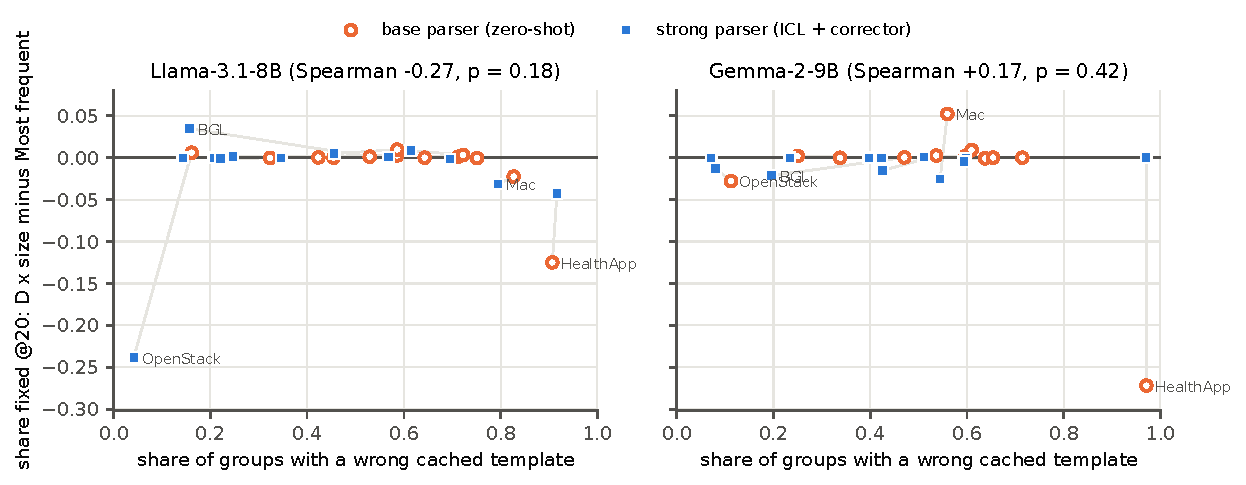
\includegraphics[width=\textwidth]{figures/strong_gap.pdf}
\caption{Does risk prediction pay off when the cached parser is more accurate? Per system, the share of mis-parsed lines fixed after 20 reviews by our transfer prior (risk $\times$ lines) minus that of reviewing the most frequent groups first (mean over 5 seeds), against the share of Drain groups whose cached template is wrong. Circles: zero-shot parser; squares: the same model with in-context demonstrations from its own cache, 10 verified seed templates and AdaParser's corrector. Lines join a system's two parsers. Points above zero favour risk prediction.}
\label{fig:strong-gap}
\end{figure*}
